\section{Introduction}
\begin{figure}[ht]
    \centering
    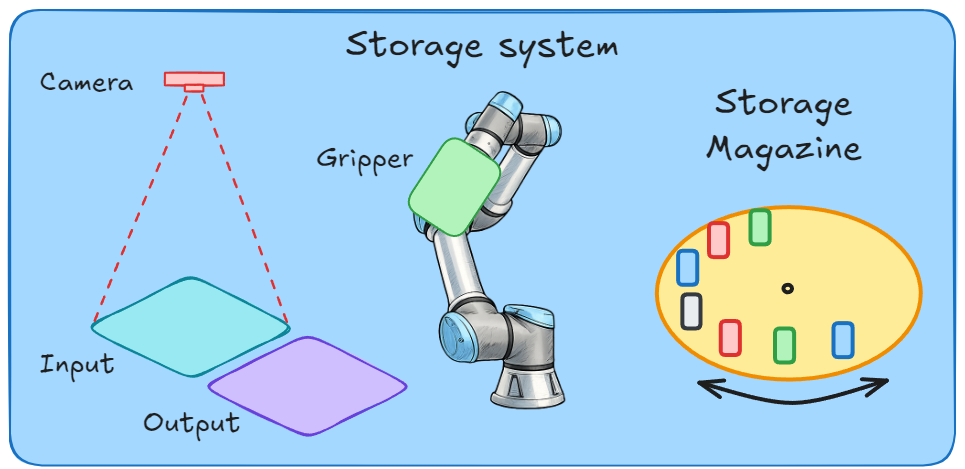
\includegraphics[width=0.8\textwidth]{figures/Early design.png}
    \caption{Early design sketch of the system}
    \label{fig:early-design}
\end{figure}


Autonomous robotic systems are increasingly used to perform repetitive tasks where reliability, cordination and accurate positioning are important. An example could be automated storage and retrieval, where objects must be identified, picked up, transported, stored, and later returned without direct human intervention. This type of system requires several technical areas to work and communicate together.
%, including computer vision, robot motion control, gripping, storage management, and communication between hardware and software.

This project focuses on the development of a prototype robotic storage and retrieval system. The system is designed around a UR5 robot arm, a custom gripper, a rotating storage disk, a camera-based vision system and a central PC program that coordinates the complete workflow. The camera is used to locate and identify objects, the robot arm moves objects between the input area and the storage system, the gripper handles the physical grasping and release of objects, and the storage disk provides multiple storage positions.
All integrated into a combined system with the PC at its center to coordinate actions and communication.
The final system is therefore evaluated as both individual subsystems and as one combined robot cell.

%The purpose of the project is not only to make the individual subsystems function separately, but also to integrate them into a complete workflow. This includes handling communication between the PC and the hardware, determining object positions, moving the robot safely and repeatably, gripping objects reliably, and keeping track of which storage positions are occupied. The final system is therefore evaluated both as a collection of subsystems and as one combined robot cell.




\subsection{Problem Statement}

This project investigates the development of a prototype of a robotic storage and retrieval system capable of autonomously identifying, picking up, storing, and retrieving physical objects. The system must therefore coordinate object localization, robot movement, grasping, and storage management to complete system. The objective of the project is to design and evaluate a prototype scale system capable of reliable object handling and storage using a robotic manipulator and custom developed  subsystems.